% Vi benytter os af MEMOIR (pr. daleif's anbefaling)
\documentclass[a4paper,11pt,oneside]{memoir}

% Dette er hovedfilen, hvor jeg definerer min pre-amble.
% Idéen er at sprede de enkelte kapitler ud i hvert deres
% dokument for at gøre det hele lidt mere overskueligt.
% Eventuelle makroer vil også fremgå heri.
% Inden 6 måneder skulle det gerne ligne et bachelorprojekt. 
% 24.01.2013

% Matematikpakker
\usepackage{amsmath}
\usepackage{amsfonts}
\usepackage{amssymb}
\usepackage{amsthm}

% Image stuff
\usepackage{graphicx}

% Dansk babel og tillad øæå osv.
\usepackage[danish]{babel}
\usepackage[utf8]{inputenc}

% Til referencer, Biber giver os UTF-8 understøttelse
\usepackage[backend=biber]{biblatex}
\usepackage{csquotes} 

% Filen med vores referencer
\addbibresource{referencer.bib}


% Styling for sætninger osv., er valgt efter normal anbefaling
\theoremstyle{plain}
\newtheorem{theorem}{Sætning}
\newtheorem{proposition}{Proposition}
\newtheorem{lemma}{Lemma}
\newtheorem{corollary}{Korollar}

\theoremstyle{definition}
\newtheorem{definition}{Definition}
\newtheorem{remark}{Bemærkning}
\newtheorem{example}{Eksempel}
\newtheorem{algorithm}{Algoritme}

% section som chapterstyle er mindre voldsomt til et "lille" projekt
% \chapterstyle{section}

% Sørg for at niveauet til og med subsection nummereres
\setcounter{secnumdepth}{2}
\setcounter{tocdepth}{1}

% TikZ bruges til tegninger
\usepackage{tikz}

% -- START PÅ MAKROER -- 
% Angiver punktet i uendelighed
\newcommand{\infp}{\mathcal{O}}

% Skriver LCM med tekst
\newcommand{\lcm}{\mathrm{LCM}}

% Hurtig måde at lave modulo
\newcommand{\modu}[1]{\ (\mathrm{mod} \ #1)}

% Lukninger af mængder
\newcommand{\clfq}{\overline{\mathbb{F}}_q}
\newcommand{\clk}{\overline{K}}

% Karakteristik
\newcommand{\cha}{\text{char}}

% -- SLUT PÅ MAKROER --

% Bruges kun under skrivningen af projektet
\includeonly{gruppeloven}

\begin{document}
% \tableofcontents
\chapter{Elliptiske kurver}
I dette kapitel vil vi introducere elliptiske kurver.
Det viser sig, at være muligt at påføre de elliptiske kurver en gruppestruktur ved en geometrisk addition af punkter fra en sådan kurve. Vi vil indføre denne additionslov og vise, at det resulterer i en abelsk gruppe. For at kunne gøre dette skal vi desuden anvende projektiv geometri, som også vil blive introduceret.

\section{Definition af elliptiske kurver}
Det er muligt at definere elliptiske kurver på flere måder. For et legeme $K$ vil følgende definition være tilstrækkelig til vores formål:
\begin{definition}
En elliptisk kurve $E$ er grafen for en ligning
\begin{align}
	\label{elliptic_curve}
	y^2 = x^3 + Ax + B,
\end{align}
hvor $A, B \in K$ er konstanter og $4A^3 + 27B^2 \neq 0$. 
\end{definition}
Vi siger, at den elliptiske kurve $E$ er på Weierstrass normalform, når den kan beskrives som i \eqref{elliptic_curve}. Hvis $\cha (K) \neq 2, 3$ er det altid muligt, at omskrive en elliptisk kurve til Weierstrass normalform (se \cite[kapitel~2]{Washington}). Det kan vises, at diskriminanten for \eqref{elliptic_curve} er \begin{align*}
	\Delta = -16(4A^3 + 27B^2),
\end{align*}
så en elliptisk kurve kan ikke have multiple rødder pr. kravet i definitionen. I figur \ref{figure_elliptic_curves} ses to eksempler på elliptiske kurver over de reelle tal.
\begin{figure}
\label{figure_elliptic_curves}
\centering
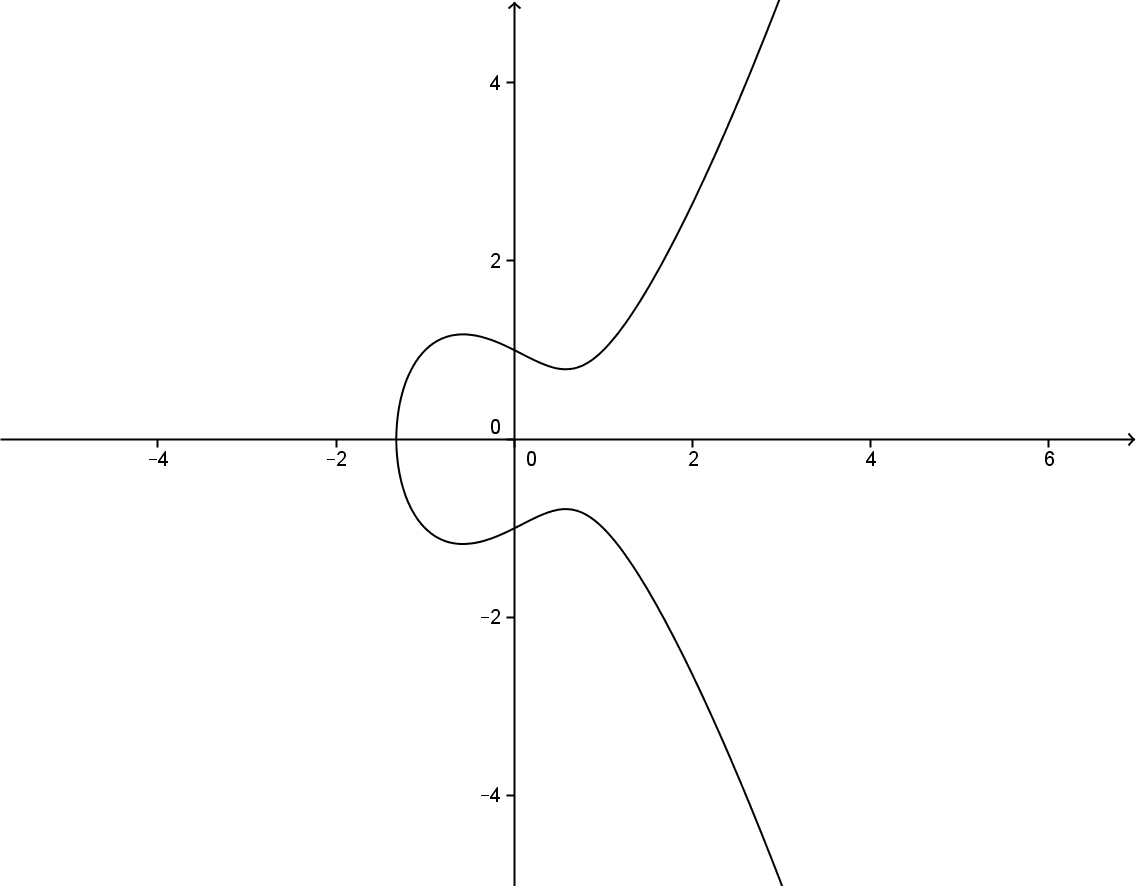
\includegraphics[scale=0.2]{elliptic_1}
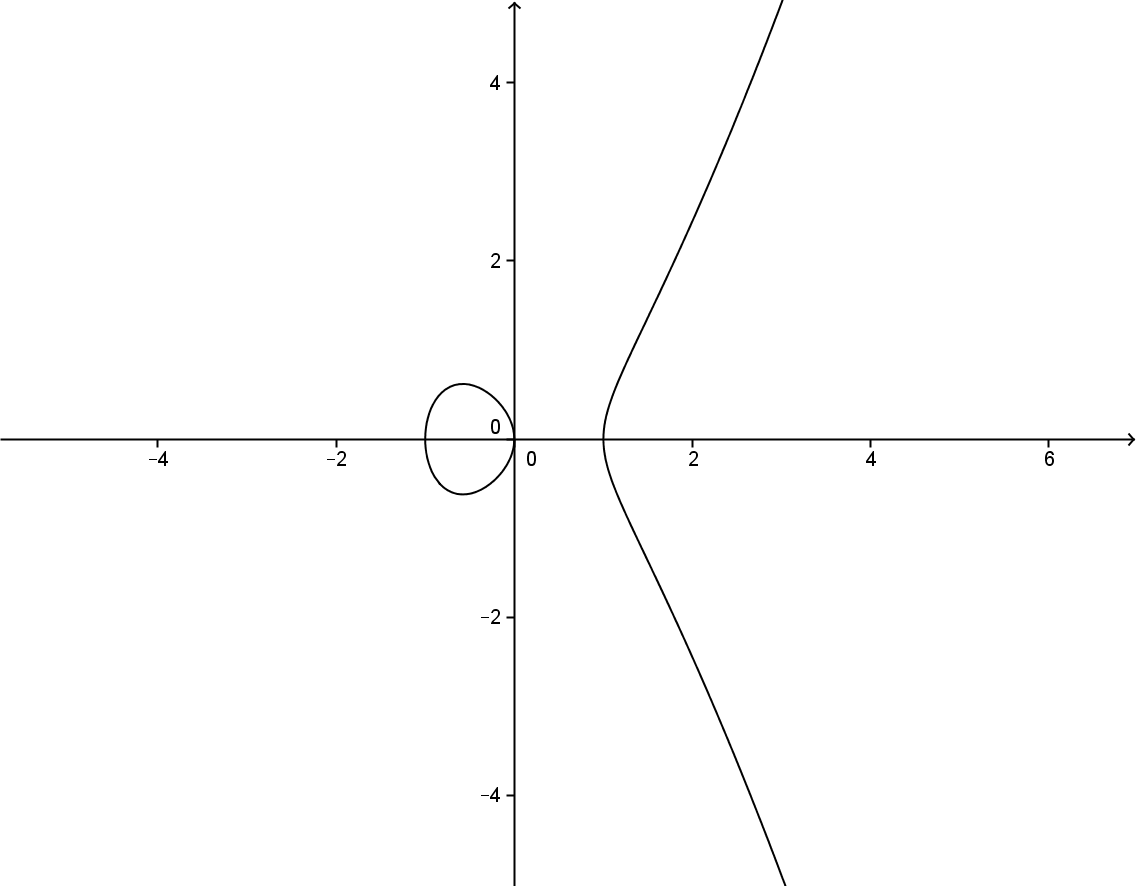
\includegraphics[scale=0.2]{elliptic_2}
\caption{Eksempler på elliptiske kurver over $\mathbb{R}$. Venstre: $y^2 = x^3 - x$, Højre: $y^2 = x^3 -x + 1$}
\end{figure}
Definitionen siger, at $A$ og $B$ skal tilhøre et legeme $K$. Det kunne f.eks. være $\mathbb{R}, \mathbb{C}$ eller $\mathbb{Q}$. Vi vil dog dog fokusere på de endelige legemer $\mathbb{F}_p = \mathbb{Z}/p\mathbb{Z}$ hvor $p$ er et primtal, og de endelige legemer med $q$ elementer $\mathbb{F}_q$, hvor $q = p^r$ for $r \geq 1$ (se appendiks \ref{appendiks_legemer}). Hvis $A, B \in K$ for en elliptisk kurve $E$ siger vi, at $E$ er givet over $K$. Fremover menes en elliptisk kurve på Weierstrass normalform, når vi snakker om en elliptisk kurve $E$. 
Punkterne på en elliptisk kurve med koordinater i et legeme $L \supseteq K$ skriver vi som $E(L)$, hvor 
\begin{align}
\label{elliptic_curve_points}
	E(L) = \{ \infty \} \cup \{ (x, y) \in L \times L \mid y^2 = x^3 + Ax + B \}.
\end{align}
Punktet $\infty$ kaldes punktet i uendelig og viser sig nødvendigt for at $E(L)$ bliver en gruppe under additionen vi introducerer i næste afsnit. Intuitivt kan vi se $\infty$ som værende punktet $(\infty, \infty)$, som er placeret i toppen af $y$-aksen. En linje siges at gå igennem $\infty$ præcist når den er lodret, hvilket betyder at to lodrette linjer skærer hinanden i $\infty$. $\infty$ kan også tænkes som værende i bunden af $y$-aksen, men så vil to lodrette linjer skære hinanden to steder, hvilket er hvorfor vi kræver at punktet $\infty$ i toppen og i bunden er et og samme punkt.

\section{Den projektive plan}
Vi vil i dette afsnit formalisere punktet $\infty$, som vi kort diskuterede ovenfor. For atk unne gøre dette får vi brug for den projektive plan 
$\mathbb{P}^2$. Rent intuitivt kan man se den projektive plan, som
værende den affine plan 
\begin{align*}
	\mathbb{A}^2(K) = \{ (x, y) \in K \times K \},
\end{align*}
hvor $K$ et et legeme, med en ekstra linje "i uendelig". 
Vi ønsker at formalisere dette begreb. 
For $x, y, z \in K$ ikke alle nul og $\lambda \in K$, $\lambda \neq 0$, 
definerer vi en ækvivalensrelation. To tripler $(x_1, y_1, z_1)$ og 
$(x_2, y_2, z_2)$ siges at være ækvivalente hvis 
\begin{align*}
	(x_1, y_1, z_1) = (\lambda x_2, \lambda y_2, \lambda z_2),
\end{align*}
og vi skriver $(x_1, y_1, z_1) \sim (x_2, y_2, z_2)$. Vi vil fremover skrive
$(x:y:z)$ for en sådan ækvivalensklasse. Den projektive plan er da givet ved
\begin{align*}
	\mathbb{P}^2(K) = \{ (x, y, z) \in K^3 \mid (x, y, z) \neq (0, 0, 0)\}/\sim.
\end{align*}
I de tilfælde hvor $z \neq 0$ har vi, at
\begin{align*}
	(x : y : z) = (x/z : y/z : 1),
\end{align*}
hvilket er de punkter vi kalder for de endelige punkter i $\mathbb{P}^2(K)$.
Vi er nemlig i stand til at associere et punkt fra $\mathbb{A}^2(K)$ med et sådan
punkt. Vi har en inklusion $\mathbb{A}^2(K) \hookrightarrow \mathbb{P}^2(K)$ givet ved
\begin{align*}
	(x, y) \mapsto (x : y : 1).
\end{align*}
Dette kan vi selvfølgelig ikke gøre, når $z=0$ og når dette er tilfældet ser vi det som, at enten $x$ eller $y$-koordinaten er $\infty$. Vi kalder dermed punkterne
$(x, y, 0)$ for punkterne i uendelig og punktet $\infty$ på en elliptisk kurve vil vi identificere med netop ét af disse.

Et polynomium siges at være homogent af grad $n$, hvis det er summen af led på formen $ax^i y^j z^k$, hvor $a \in K$ og $i + j + k = n$. Eksempelvis er 
\begin{align*}
	F(x, y, z) = 5x^4 - 2x^2 yz + 7yz^3
\end{align*}
et homogent polynomium af grad $4$. For et homogent polynomium $F$ af grad $n$ er
\begin{align*}
	F(\lambda x, \lambda y, \lambda z) = \lambda^n F(x, y, z), \quad \lambda \in K.
\end{align*}
Vi har altså, at når $(x_1, y_1, z_1) \sim (x_2, y_2, z_2)$ er $F(x_1, y_1, z_1) = 0$ hvis og kun hvis $F(x_2, y_2, z_2) = 0$. Et nulpunkt for $F$ i $\mathbb{P}^{2}(K)$ er altså ikke afhængig af repræsentanten for en given ækvivalensklasse, hvilket betyder at nulpunkterne for $F$ er veldefineret i $\mathbb{P}^{2}(K)$.

For et arbitrært polynomium $F(x, y, z)$ giver det ikke mening, at snakke om et punkt i $\mathbb{P}^2(K)$ hvor $F(x, y, z) = 0$, da det nemlig afhænger af repræsentanten $(x, y, z)$ for ækvivalensklassen. Vi har f.eks., at for
$F(x, y, z) = 2x^2 - y - z$ at $F(1, 1, 1) = 0$, men $F(2, 2, 2) = 4$. Men da $(1 : 1 : 1) = (2 : 2 : 2)$ har vi et problem, som vi undgår ved at arbejde med homogene polynomier i stedet. For et polynomium $f(x, y)$ kan vi homogenisere det ved, at indsætte de korrekte potenser af $z$. F.eks. for $f(x, y) = y^2 - x^3 - Ax - B$ har vi, at $F(x, y) = y^2 z - x^3 - Axz^2 - Bz^3$. Generelt for et polynomium $f(x, y)$ har vi at, hvis
\begin{align*}
	f(x, y) = \sum_{i} a_i x^{p_i} y^{q_i},
\end{align*}
hvor $\max \{p_i + q_i \} = n$, er dets homogene form
\begin{align*}
	F(x, y, z) = \sum_i a_i x^{p_i} y^{q_i} z^{n-p_i - q_i}.
\end{align*}
Dermed har vi, at 
\begin{align*}
	F(x, y, z) &= z^n \sum_i a_i x^{p_i} z^{-p_i} y^{q_i} z^{-q_i} = z^n \sum_i a_i \left( \frac{x}{z} \right)^{p_i}
	\left( \frac{y}{z} \right)^{q_i} \\  
	&= z^n f\left( \frac{x}{z}, \frac{y}{z} \right).
\end{align*}
Da er det klart, at 
\begin{align*}
	f(x, y) = F(x, y, 1).
\end{align*}
Vi er nu i stand til at undersøge, hvad det vil sige for to parallelle linjer at mødes i uendelig. Lad først
\begin{align*}
	y = mx + b_1, \quad y = mx + b_2,
\end{align*}
være to linjer, som ikke er lodrette og hvor $b_1 \neq b_2$. Homogeniserer vi dem, som forklaret ovenfor, får vi
\begin{align*}
	y = mx + b_1z, \quad y = mx + b_2 z.
\end{align*}
Trækker vi ligningerne fra hinanden får vi, at 
\begin{align*}
	0 = (b_1 - b_2)z \Rightarrow z = 0,
\end{align*}
hvilket så betyder, at $y = mx$. Da vi ikke kan have, at både $x, y$ og $z$ er $0$ samtidigt må vi have $x \neq 0$. Vi kan da dele med $x$ og vi får, at skæringen er
\begin{align*}
	(x : mx : 0) = (1 : m : 0).
\end{align*}
Dette er et af punkterne i uendelig fra $\mathbb{P}^2(K)$.
På samme måde har vi, at hvis $x=c_1$ og $x=c_2$ er lodrette linjer, at de skærer hinanden i punktet $(0 : 1 : 0)$. Dette er også ét af de punkter, som vi identificerede som værende et punkt i uendelig i $\mathbb{P}^2(K)$.

Hvis vi nu homogeniserer ligningen for en elliptisk kurve $E$ med variablen $z$ får vi, at
\begin{align*}
\label{homogeniseret_weierstrass}
	y^2 z = x^3 + Ax z^2 + B z^3.
\end{align*} 
For at se hvilke punkter i uendelig, som er på $E$ sætter vi $z=0$. Dette giver os, at $0 = x^3$ hvilket har en tredobbelt rod i $x=0$ og $y$ kan være et hvilket som helst tal som ikke er $0$, da vi ikke kan have $(0 : 0 : 0)$. 
Efter en skalering med $y$ har vi $(0 : y : 0) = (0 : 1 : 0)$ så $(0 : 1 : 0)$ er det eneste punkt i uendelig på $E$. Da $(0 : 1 : 0)$ er et punkt på enhver lodret linje skærer enhver lodret linje $E$ i dette punkt i uendelig. Vi har desuden, da $(0 : 1 : 0) = (0 : -1 : 0)$, at punkterne i uendelig i toppen og bunden af $y$-aksen er de samme.

Vi vil dog her foretrække, at arbejde med affine koordinater, hvor punktet $\infty$ behandles som et specialtilfælde, men vi har nu givet konkret mening til punktet $\infty$.

\section{Gruppeloven}
Lad $E$ være en elliptisk kurve over et legeme $K$. Det viser sig, at vi kan tage to punkter (eller blot ét) på $E$ og producere et tredje punkt som også er på $E$. Vi vil i dette afsnit vise, hvordan dette gøres og til slut konkludere, at defineres dette som en additions operator bliver $E(K)$ en additiv abelsk gruppe. Vælg to punkter
\begin{align*}
	P_1 = (x_1, y_1) \quad \text{og} \quad P_2 = (x_2, y_2)
\end{align*}
på $E$. 
\begin{figure}
\label{figure_addition_law}
\centering
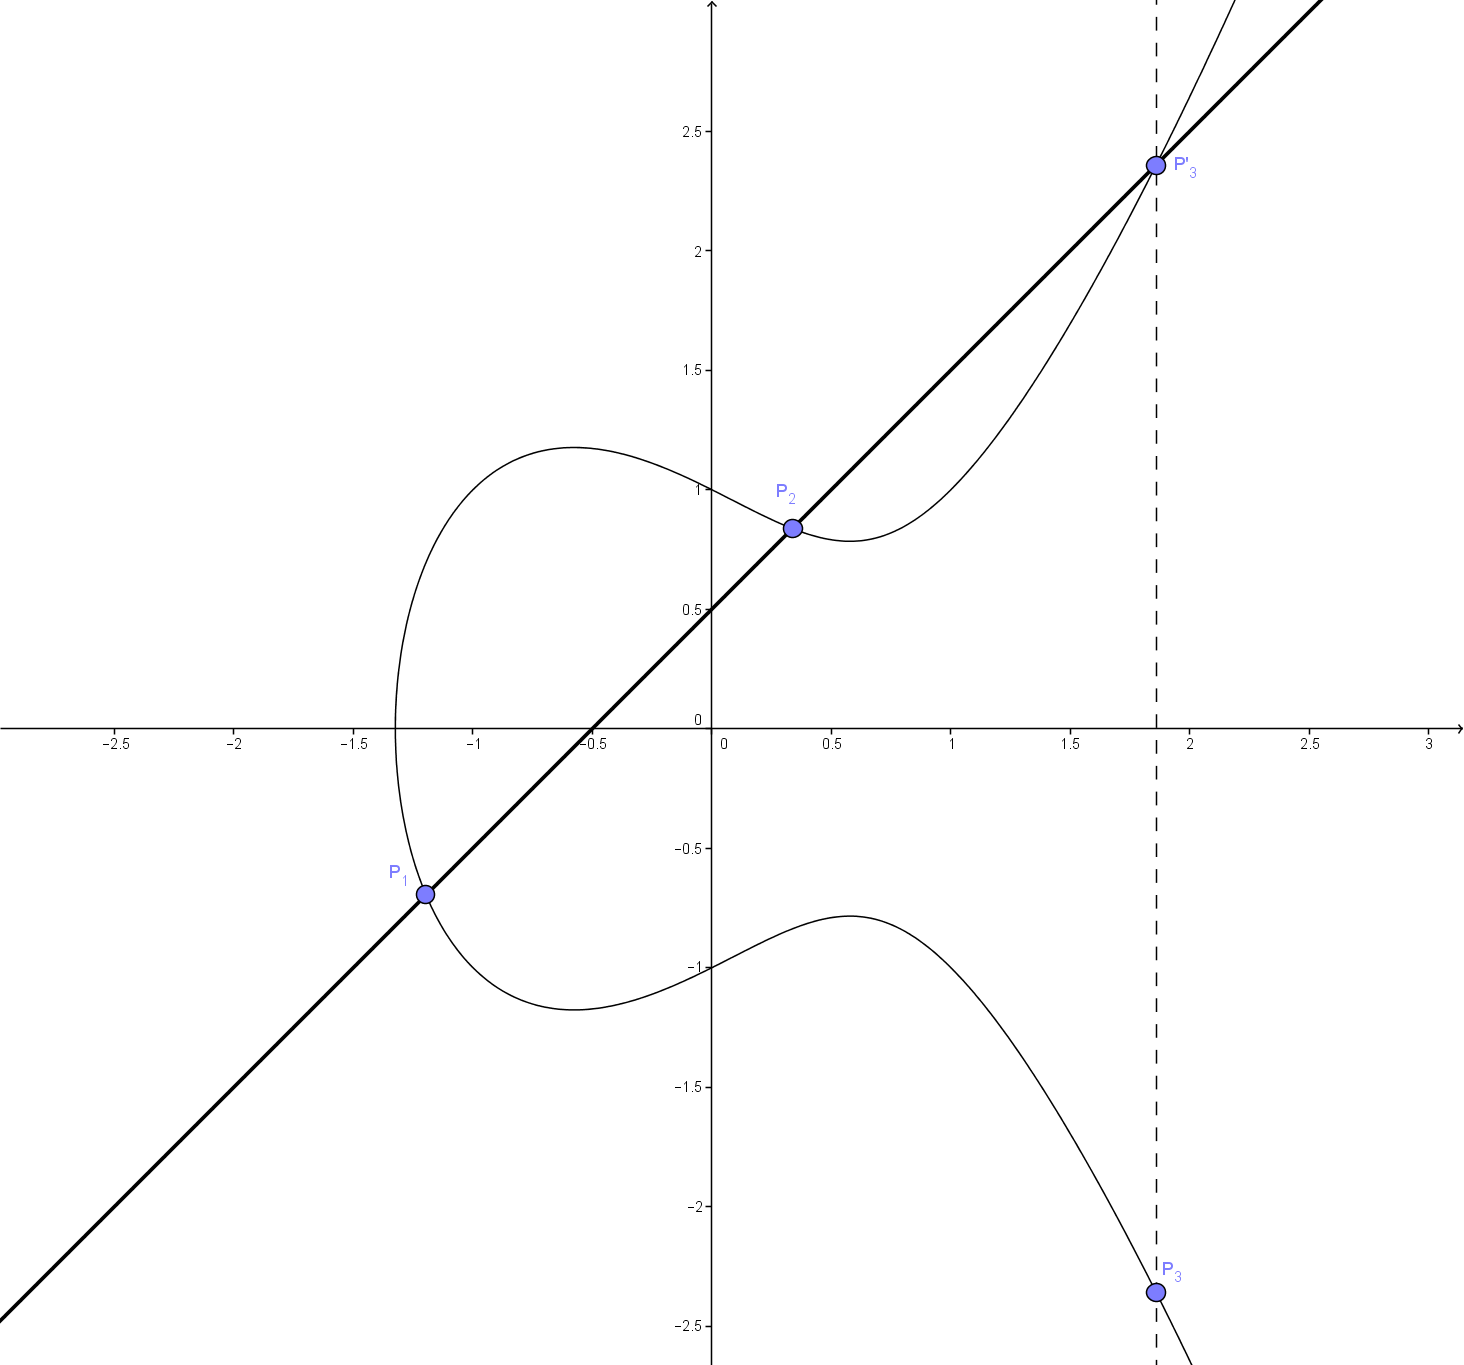
\includegraphics[scale=0.25]{elliptic_3}
\caption{Addition af to punkter på en elliptisk kurve}
\end{figure}
Vi kan da trække en ret linje $L$ igennem punkterne $P_1$ og $P_2$, som så vil skære kurven for $E$ i et tredje punkt ${P_3}'$ (se appendiks for bevis om skæring i 3 punkter). Vi definerer $P_1 + P_2 = P_3$ til at være reflektionen i $x$-aksen af dette punkt. 

Vi vil nu udlede formlerne for denne addition af punkter på $E$. Antag først, at $P_1 \neq P_2$ og lad $P_1$ og $P_2$ være forskellige fra $\infty$. Vi har da, at hældningen for linjen der går igennem $P_1$ og $P_2$ er
\begin{align*}
	m = \frac{y_2 - y_1}{x_2 - x_1}.
\end{align*}
Hvis $x_1 = x_2$ er linjen lodret, hvilket er et tilfælde som vi behandler senere. Antag altså at $x_1 \neq x_2$, vi har da
\begin{align*}
	y_2 = m(x_2 - x_1) + y_1.
\end{align*}
Vi indsætter dette i ligningen for $E$ og får, at 
\begin{align*}
	(m(x-x_1) + y_1)^2 = x^3 + Ax + B.
\end{align*}
Skrives dette ud får vi, at
\begin{align*}
	0 &= x^3 + Ax + B - 2y_1 m(x-x_1) - m^2 (x - x_1)^2 - y_{1}^{2} \\
	&= x^3 + Ax + B - 2y_1 m x - 2y_1 m x_1 - m^2 (x^2 -2x x_1 + x_{1}^{2}) - y_{1}^{2} \\
	&= x^3 - m^2 x^2 + (A-2my_1 +2m^2x_1)x -2m y_1 x_1 -m^2 x_{1}^{2} - y_{1}^{2} + B. 
\end{align*}
Denne har tre rødder, som netop er de tre punkter, hvor $L$ skærer $E$.
Pr. vores konstruktion kender vi allerede de to rødder $x_1$ og $x_2$,
og vi ønsker at finde den tredje. Generelt for et kubisk polynomium 
$x^3 + ax^2 + bx + c$, med rødder $r, s, t$, har vi at 
\begin{align*}
	x^3 + ax^2 + bx + c = (x - r)(x - s)(x - t) = x^3 - (r + s + t)x^2 + \ldots,
\end{align*}
hvilket giver os, at $-a = r + s + t$. Hvis de to rødder vi kender er $r$ og $s$
kan vi finde den sidste som
\begin{align*}
	t = -a - r - s.
\end{align*}
I vores tilfælde er $a=-m^2$ så vi har, at 
\begin{align*}
	x = m^2 - x_1 - x_2.
\end{align*}
Vi mangler da blot at reflektere dette punkt for at have fundet 
punktet $P_1 + P_2 = P_3 = (x, y)$. Vi reflekterer over $x$-aksen og finder, at 
\begin{align*}
	x = m^2 - x_1 - x_2, \quad y = m(x_1 - x) - y_1.
\end{align*}
Vi vender nu tilbage til tilfældet, hvor $x_1 = x_2$. Da vil linjen igennem 
$P_1$ og $P_2$ være lodret, så den skærer $E$ i $\infty$. Vi husker, at når $\infty$ 
reflekteres over $x$-aksen får vi igen $\infty$. Vi får altså, at $P_1 + P_2=\infty$.

Tilfældet hvor $P_1 = P_2 = (x_1, y_1)$ kræver lidt flere overvejelser. For to punkter som ligger
tæt på hinanden vil linjen igennem punkterne nærme sig tangenten til et af punkterne. Når vi har to ens punkter lader vi da linjen igennem dem være tangenten til punktet. Ved implicit differentiation finder vi, at 
\begin{align*}
	2y \frac{dy}{dx} = 3x^2 + A, \quad \text{så} \quad m = \frac{dy}{dx} = \frac{3x_{1}^{2} + A}{2y_1}.
\end{align*}
Hvis $y_1 = 0$ er linjen lodret og i det tilfælde lader vi $P_1 + P_2 = \infty$. Antag altså, at $y_1 \neq 0$. Ligningen for $L$ er 
\begin{align*}
	y = m(x-x_1) + y_1,
\end{align*}
som før. Vi får den kubiske ligning
\begin{align*}
	0 = x^3 - m^2 x^2 + \ldots
\end{align*}
Vi kender dog kun én rod, $x_1$, men den er en dobbelt rod idet at $L$ er tangent til $E$ i $P_1$. Så på samme måde som før får vi, at 
\begin{align*}
	x_3 = m^2 - 2x_1, \quad y_3 = m(x_1 - x_3) - y_1.
\end{align*}
Antag nu, at $P_2 = \infty$. Linjen som går igennem $P_1$ og $\infty$ er en lodret linje, som skærer $E$ i reflektionen af $P_1$ over $x$-aksen. Når vi reflekterer dette punkt igen over $x$-aksen får vi igen $P_1$. Altså har vi, at
\begin{align*}
	P_1 + \infty = P_1.
\end{align*}
Denne definition udvides sådan, at $\infty + \infty = \infty$.

Det er nu mere klart, hvorfor elliptiske kurver og denne definition for en addition passer sammen. Højresiden i en ligning på Weierstrass normalform er kubisk så en linje igennem to punkter skærer den i et tredje punkt. At venstresiden er $y^2$ sikrer os, at kurven er symmetrisk om $x$-aksen, som benyttes når vi reflekterer et punkt. Vi opsummerer denne diskussion og kan opstille gruppeloven:

\begin{definition}[Gruppeloven]
\label{gruppeloven:definitionen}
Lad $E$ være en elliptisk kurve. Givet to punkter, $P_1, P_2 \in E(K)$, $P_i = (x_i, y_i)$, findes et tredje punkt $P_3 = P_1 + P_2 = (x_3, y_3)$ da som følger
\begin{enumerate}
	\item Hvis $x_1 \neq x_2$ er 
	\begin{align*}
		x_3 = m^2 - x_1 - x_2, \quad y_3 = m(x_1 - x_3) - y_1,
	\end{align*}		
	hvor $m = (y_2 - y_1)/(x_2 - x_1)$.
	\item Hvis $x_1 = x_2$, men $y_1 \neq y_2$ da er $P_1 + P_2 = \infty$.
	\item Hvis $P_1 = P_2$ og $y_1 \neq 0$ er 
	\begin{align*}
		x_3 = m^2 - 2x_1, \quad y_3=m(x_1 - x_3) - y_1,
	\end{align*}
	hvor $m=(3{x_1}^2 + A)/2y_1$.
	\item Hvis $P_1 = P_2$ og $y_1 = 0$ da er $P_1 + P_2 = \infty$.
\end{enumerate}
Vi definerer desuden, at 
\begin{align*}
	P + \infty = \infty,
\end{align*}
for alle $P \in E(K)$.
\end{definition}
Det måske overraskende hovedresultatet i dette kapitel er, at denne addition resulterer i en abelsk gruppe:

\begin{thm}
Punkterne på $E$, altså $E(K)$, udgør en additiv abelsk gruppe hvor $\infty$ er identiteten og additionen er som defineret i gruppeloven. 
\end{thm}
\begin{proof}
For at være en gruppe skal additionen af punkter være kommutativ, der skal eksistere en identitet, hvert element skal have en invers og additionen af punkter skal være associativ.

Kommutativiteten kan enten ses direkte fra formlerne eller fra det faktum, at linjen igennem $P_1$ og $P_2$ er den samme som linjen igennem $P_2$ og $P_1$. At $\infty$ er identiteten følger pr. definitionen af denne. For de inverse elementer lader vi $P'$ være reflektionen af $P$, da er $P+P' = \infty$. Associativiteten kan vises direkte ud fra formlerne, men der er mange tilfælde der skal behandles, hvilket gør det besværligt. Et bevis for associativiteten kan findes i \cite[afsnit~2.4]{Washington} eller i \cite{Silverman}.
\end{proof}
\chapter{Endomorfier}
Vi vil i dette kapitel etablere nogle vigtige resultater vedrørende endomorfier på elliptiske kurver, som viser sig nødvendige i beviset for Hasses sætning.

\section{Endomorfier på elliptiske kurver}
Lad $K$ være et legeme og $\clk$ dens tilhørende algebraiske aflukning. I det følgende vil vi med en elliptisk kurve $E$ mene en kurve på formen $y^2 = x^3 + Ax + B$. 
Vi begynder da med følgende definition:

\begin{definition}
En endomorfi på $E$ er en homomorfi $\alpha : E(\clk) \to E(\clk)$ givet
ved rationale funktioner.
\end{definition}

Med en rational funktion forstår vi en kvotient af polynomier. Det vil altså sige, at 
en endomorfi $\alpha$ skal opfylde, at $\alpha(P_1 + P_2) = \alpha(P_1) + \alpha(P_2)$ 
og der skal findes rationale 
funktioner $R_1(x, y)$ og $R_2(x, y)$, begge med koefficienter i $\clk$, så
\begin{align*}
	\alpha(x, y) = (R_1(x, y), R_2(x, y)),
\end{align*}
for alle $(x, y) \in E(\clk)$. da $\alpha$ er en homomorfi gælder der, at $\alpha(\infty)=\infty$. Den trivielle endomorfi angives med $0$ og er den endomorfi, som sender ethvert punkt til $\infty$. Vi vil fremover antage, at $\alpha$ ikke er den trivielle endomorfi, hvilket betyder at der findes $(x, y)$ sådan at $\alpha(x, y) \neq \infty$.

\begin{example}
Lad $E$ være en elliptisk kurve og lad $\alpha$ være givet ved, at $\alpha(P)=2P$. Da er $\alpha$ en homomorfi og
$\alpha(x, y) = (R_1(x, y), R_2(x, y))$, hvor
\begin{align*}
	R_1(x, y) &= \left( \frac{3x^2 + A}{2y} \right)^2 - 2x, \\
	R_2(x, y) &= \left( \frac{3x^2 + A}{2y} \right) \left(x - \left( \left( \frac{3x^2 + A}{2y} \right)^2 - 
	2x \right) \right) - y \\
	&= \left( \frac{3x^2 + A}{2y} \right) \left(3x - \left( \frac{3x^2 + A}{2y} \right)^2 \right) - y.
\end{align*}
Da både $R_1$ og $R_2$ er rationale funktioner er $\alpha$ en endomorfi for $E$.
\end{example}


Vi ønsker nu, at finde en standard repræsentation for de rationale funktioner, som en endomorfi er givet ved. Følgende sætning gør dette muligt for os:

\begin{thm}
\label{end_rep_theorem}
Lad $E$ være en elliptisk kurve over et legeme $K$. En endomorfi $\alpha$ kan da skrives som
\begin{align*}
	\alpha(x, y) = (r_1(x), r_2(x)y) = \left( \frac{p(x)}{q(x)}, \frac{s(x)}{t(x)}y \right),
\end{align*}
hvor $p, q$ henholdsvis $s, t$ ikke har nogen fælles faktor.
\end{thm}
\begin{proof}
For et punkt $(x, y) \in E(\clk)$ gælder der, at $y^2 = x^3 + Ax + B$ så vi har også, at 
\begin{align*}
	y^{2k} = (x^3 + Ax + B)^k \quad \text{og} \quad y^{2k+1}= y^{2k}y = (x^3 + Ax + B)^k y, \quad k \in \mathbb{N}.
\end{align*}
Vi kan altså erstatte en lige potens af $y$ med et polynomium der kun afhænger af $x$, og en ulige potens med $y$ ganget med et polynomium der kun afhænger af $x$. For en rational funktion $R(x, y)$ kan vi da beskrive en anden rational funktion, som stemmer overens med denne på punkter fra $E(\clk)$. Vi kan altså antage, at
\begin{align}
	\label{rational_1}
	R(x, y) = \frac{p_1(x) + p_2(x)y}{p_3(x)+p_4(x)y}.
\end{align}
Vi kan endda gøre det endnu simplere ved at gange udtrykket i \eqref{rational_1} med $p_3(x)-p_4(x)$, hvilket giver 
\begin{align*}
	(p_3(x) - p_4(x)y)(p_3(x)+p_4(x)y) = p_3(x)^2 - p_4(x)^2 y^2,
\end{align*}
hvorefter vi kan erstatte $y^2$ med $x^3 + Ax + B$. Dette giver os altså, at 
\begin{align}
	\label{rational_final}
	R(x, y) = \frac{q_1(x) + q_2(x)y}{q_3(x)}.
\end{align}
Da $\alpha$ er en endomorfi er den givet ved
\begin{align*}
	\alpha(x, y) = (R_1(x, y), R_2(x, y)),
\end{align*}
hvor $R_1$ og $R_2$ er rationale funktioner. Da $\alpha$ specielt er en homomorfi bevarer den strukturen for en elliptisk kurve så vi har, at
\begin{align*}
	\alpha(x, -y) = \alpha(-(x, y)) =  -\alpha(x, y).
\end{align*}
Dette medfører, at 
\begin{align*}
	R_1(x, -y) = R_1(x, y) \quad \text{og} \quad R_2(x, -y) = -R_2(x, y).
\end{align*}
Skriver vi $R_1$ på samme form som i \eqref{rational_final} må $q_2(x) = 0$, og ligeledes må vi for $R_2$ have at $q_1(x) = 0$. Vi kan altså antage, at
\begin{align*}
		\alpha(x, y) = (r_1(x), r_2(x)y),
\end{align*}
hvor $r_1(x)$ og $r_2(x)$ er rationale funktioner. Skriv da
\begin{align*}
	r_1(x) = \frac{p(x)}{q(x)} \quad \text{og} \quad r_2(x)=\frac{s(x)}{t(x)}y,
\end{align*}
hvor $p, q$ henholdsvis $s, t$ ikke har nogen fælles faktorer. Hvis $q(x)=0$ for et punkt $(x, y)$ lader vi 
$\alpha(x, y) = \infty$. Hvis $q(x) \neq 0$ giver (ii) i lemma \ref{rational_lemma}, at $r_2(x)$ da også vil være defineret.
\end{proof}

\begin{lemma}
\label{rational_lemma}
Lad $\alpha$ være en endomorfi givet ved
\begin{align*}
	\alpha(x, y) = \left( \frac{p(x)}{q(x)}, \frac{s(x)}{t(x)}y \right),
\end{align*}
for en elliptisk kurve $E$. Lad $p, q$ henholdsvis $s, t$ være sådan, at de ikke har nogen fælles rødder. Da har vi, at
\begin{enumerate}[(i)]
	\item For et polynomium $u(x)$, som ikke har en fælles rod med $q(x)$ har vi, at
	\begin{align*}
		\frac{(x^3+Ax+B)s(x)^2}{t(x)^2} = \frac{u(x)}{q(x)^3}.
	\end{align*}
	\item $t(x_0)=0$ hvis og kun hvis $q(x_0)=0$.
\end{enumerate}
\end{lemma}
\begin{proof}
(i) For et punkt $(x, y) \in E(K)$ har vi også, at $\alpha(x, y) \in E(K)$, da $\alpha$ er en endomorfi. Derfor har vi, at
\begin{align*}
	\frac{(x^3 + Ax + B)s(x)^2}{t(x)^2} &= \frac{y^2 s(x)^2}{t(x)^2} = \left( \frac{s(x)}{t(x)}y \right)^2 \\
	&= \left( \frac{p(x)}{q(x)} \right)^3 + A \left( \frac{p(x)}{q(x)} \right) + B \\
	&= \frac{p(x)^3 + A p(x) q(x)^2 + B q(x)^3}{q(x)^3} = \frac{u(x)}{q(x)^3},
\end{align*}
hvor $u(x) = p(x)^3 + A p(x) q(x)^2 + B q(x)^3$. Antag nu, at $q(x_0)=0$. Hvis nu også $u(x_0)=0$ følger det, at
\begin{align*}
	u(x_0)=p(x_0)^3 + A p(x_0) q(x_0)^2 + B q(x_0)^3 = 0 &\Rightarrow p(x_0)^3 = 0 \\ &\Rightarrow p(x_0)=0,
\end{align*}
men $p$ og $q$ havde pr. antagelse ingen fælles rødder. Så hvis $q(x_0) = 0$ må $u(x_0) \neq 0$ og de har dermed ingen fælles rødder.

(ii) Vi ved fra (i), at 
\begin{align}
	\label{lemma_rational_sup}
	(x^3 + Ax + B)s(x)^2 q(x)^3 = u(x) t(x)^2.
\end{align}
Hvis $q(x_0) = 0$ følger det direkte fra \eqref{lemma_rational_sup}, at 
\begin{align*}
	u(x_0)t(x_0)^2 = 0.
\end{align*}
Da $q$ og $u$ ikke har nogen fælles rødder følger det, at $t(x_0) = 0$. Antag nu, at $t(x_0)=0$, da har vi fra
\eqref{lemma_rational_sup}, at
\begin{align*}
	({x_0}^3 + Ax_0 + B)s(x_0)^2 q(x_0)^3 = 0.
\end{align*}
Da $s$ og $t$ pr. antagelse ikke har nogen fælles rødder giver det yderligere, at 
\begin{align*}
	({x_0}^3 + Ax_0 + B)q(x_0)^3 = 0.
\end{align*}
Hvis ${x_0}^3 + Ax_0 + B \neq 0$ er $q(x_0)^3 = 0$ og dermed må $q(x_0) = 0$. Hvis vi derimod har, at 
${x_0}^3 + Ax_0 + B = 0$ er det klart, at $(x-x_0) \mid (x^3 + Ax + B)$. Med andre ord findes et polynomium $Q(x)$ sådan, at
\begin{align*}
	(x^3 + Ax + B) = (x-x_0)Q(x),
\end{align*}
hvor $Q(x_0) \neq 0$, da $x^3 + Ax + B$ ikke har nogen dobbeltrødder. Da $t(x_0)=0$ findes der også et polynomium $T(x)$ sådan, at
\begin{align*}
	t(x) = (x-x_0)T(x).
\end{align*}
Udtrykket fra \eqref{lemma_rational_sup} kan da skrives, som
\begin{align*}
	(x-x_0)Q(x)s(x)^2q(x)^3 = u(x) ((x-x_0)T(x))^2,
\end{align*}
hvilket med division med $(x-x_0)$ giver os, at
\begin{align*}
	Q(x)s(x)^2 q(x)^3 =  u(x) (x-x_0) T(x)^2.
\end{align*}
I tilfældet, hvor $x=x_0$ har vi så, at
\begin{align*}
	Q(x_0)s(x_0)^2q(x_0)^3 = 0,
\end{align*}
men da $Q(x_0) \neq 0$ og $s(x_0) \neq 0$ må $q(x_0)^3 = 0$ så $q(x_0)=0$.
\end{proof}


Med den nu etablerede standard repræsentation for endomorfier, er vi i stand til at give en definition for graden af en endomorfi:

\begin{definition}
Graden af en endomorfi $\alpha$ er givet ved
\begin{align*}
	\deg(\alpha) = \max \{ \deg p(x), \deg q(x) \},
\end{align*}
når $\alpha$ ikke er den trivielle endomorfi, altså for $\alpha \neq 0$. For $\alpha = 0$ lader vi $\deg (\alpha) = 0$.
\end{definition}

En endomorfi siges at være \textit{separabel} hvis den afledede $r_1'(x) \neq 0$.

Den følgende proposition er essentiel idet, at det tilknytter graden af en endomorfi til antallet af elementer i kernen for selvsamme endomorfi. Dette faktum benyttes direkte i beviset for Hasses sætning.

\begin{proposition}
\label{deg_to_ker}
Lad $E$ være en elliptisk kurve. Lad $\alpha \neq 0$ være en separabel 
endomorfi for $E$. Da er 
\begin{align*}
	\deg \alpha = \# \ker (\alpha),
\end{align*}
hvor $\ker (\alpha) = $ angiver kernen for homomorfien 
$\alpha : E(\clk) \to E(\clk)$. I tilfældet hvor $\alpha \neq 0$ ikke
er separabel gælder der, at 
\begin{align*}
	\deg \alpha > \# \ker (\alpha).
\end{align*}
\end{proposition}
\begin{proof}
Vi skriver $\alpha$ på standardformen, som vi introducerede tidligere, altså
sættes
\begin{align*}
	\alpha(x, y) = (r_1(x), r_2(x) y)),
\end{align*}
hvor $r_1(x) = p(x)/q(x)$. Da $\alpha$ er antaget til at være separabel er 
$r_1' \neq 0$ og dermed er $pq'-p'q$ ikke nulpolynomiet. Lad nu
\begin{align*}
	S = \{ x \in \clk \mid (pq' - p'q)(x)q(x) = 0 \}.
\end{align*}
Lad da $(a, b) \in E(\clk)$ være valgt sådan, at følgende er opfyldt
\begin{enumerate}
	\item $a \neq 0$, $b \neq 0$ og $(a, b) \neq \infty$,
	\item $\deg (p(x) - aq(x)) = \max \{ \deg p(x), \deg q(x) \} = \deg \alpha$,
	\item $a \notin r_1(S)$,
	\item $(a, b) \in \alpha(E(\clk))$.
\end{enumerate}
Da $pq'-p'q$ ikke er 
nulpolynomiet er $S$ en endelig mængde, hvilket dermed også betyder, at 
$\alpha(S)$ er en endelig mængde. Funktionen $r_1(x)$ antager uendeligt 
mange forskellige værdier når $x$ gennemløber $\clk$, da en algebraisk aflukning indeholder uendeligt mange elementer.
%da en algebraisk aflukning indeholder uendeligt mange elementer.
Da der for hvert $x$ er et punkt $(x, y) \in E(\clk)$ følger det, at 
$\alpha(E(\clk))$ er en uendelig mængde. Det er altså muligt, at vælge et
punkt $(a, b) \in E(\clk)$ med egenskaberne ovenfor.

Vi ønsker at vise, at der netop er $\deg \alpha$ punkter $(x_1, y_1) \in E(\clk)$ sådan,
at $\alpha(x_1, y_1) = (a, b)$. For et sådan punkt gælder der, at 
\begin{align*}
	\frac{p(x_1)}{q(x_1)} = a, \quad r_2(x_1) y_1 = b.
\end{align*}
Da $(a, b) \neq \infty$ er $q(x_1) \neq 0$. % Øvelse giver, at r_2(x_1) er defineret
Da $b \neq 0$ har vi også, at $y_1 = b / r_2(x_1)$. Dette betyder, at $y_1$ er bestemt
ved $x_1$, så vi behøver kun at tælle værdier for $x_1$. Fra antagelse (2) har vi, at 
$p(x) - aq(x) = 0$ har $\deg \alpha$ rødder talt med multiplicitet. Vi skal altså vise,
at $p-aq$ ikke har nogen multiple rødder. Antag for modstrid, at $x_0$ er en multipel
rod. Da har vi, at
\begin{align*}
	p(x_0) - aq(x_0) = 0 \quad \text{og} \quad p'(x_0) - aq'(x_0) = 0.
\end{align*}
Dette kan omskrives til ligningerne $p(x_0)=aq(x_0)$ og $aq'(x_0)=p'(x_0)$, 
som vi ganger med hinanden og får, at 
\begin{align*}
	a p(x_0)q'(x_0) = ap'(x_0)q(x_0).
\end{align*} 
Da $a \neq 0$ pr. (1) giver det os, at $x_0$ er en rod i $pq'-p'q$ så $x_0 \in S$.
Altså er $a=r_1(x_0) \in r_1(S)$, hvilket er i modstrid med (3). Dermed har 
$p-aq$ netop $\deg \alpha$ forskellige rødder. Da der er præcist $\deg \alpha$ 
punkter $(x_1, y_1)$ så $\alpha(x_1, y_1) = (a, b)$ har kernen for $\alpha$ netop
$\deg \alpha$ elementer.
\end{proof}

Dette bevis konkluderer undersøgelse af endomorfier på generelle legemer $K$. I kapitel 4
vil vi fortsat behandle endomorfier, men der vil det være for endelige legemer.



















\chapter{Elliptiske kurver over endelige legemer}

Vi skal i dette kapitel undersøge elliptiske kurver over endelige legemer. 
Lad $\mathbb{F}$ være et endeligt legeme og lad $E$ være en elliptisk kurve på
formen 
\begin{align*}
	y^2 = x^3 + Ax + B,
\end{align*}
som er defineret over $\mathbb{F}$. Da er gruppen $E(\mathbb{F})$ endelig, da 
der kun findes endeligt mange talpar $(x, y)$ så $x, y \in \mathbb{F}$. Lad 
$E$ være den elliptiske kurve $y^2 = x^3 - x$ over $\mathbb{F}_5$. For at bestemme
ordenen af $E(\mathbb{F})$ laver vi en tabel over mulige værdier for $x$, $x^3 - x \modu{5}$
og for $y$ som er kvadratrødderne af $x^3 - x$. Dette giver os samtlige punkter på kurven:


\begin{center}
\begin{tabular}{c c c c }
$x$ & $x^3 - x$ & $y$ & Punkter \\ 
\hline
$0$ & $0$ & $0$ & $(0, 0)$ \\ 
$1$ & $0$ & $0$ & $(1, 0)$ \\ 
$2$ & $1$ & $\pm 1$ & $(2, 1), (2, 4)$ \\ 
$3$ & $4$ & $\pm 2$ & $(3, 2), (3, 3)$ \\ 
$4$ & $2$ & $-$ & $-$ \\ 
$\infty$ & & $\infty$ & $\infty$ \\
\end{tabular} 
\end{center}

Bemærk, at $\sqrt{2} \notin \mathbb{Z}$ og derfor har $2$ ikke en kvadratrod i $\mathbb{F}_5$.
Dette giver os, at $E(\mathbb{F}_5)$ har orden $7$ og vi skriver $\#E(\mathbb{F}_5)=7$. Vi skal
i dette kapitel vise Hasses sætning, som giver en vurdering for antallet af punkter på en elliptisk
kurve over et endeligt legeme:

\begin{theorem}[Hasse]
\label{hasse}
Lad $E$ være en elliptisk kurve over et endeligt legeme $\mathbb{F}_q$. Da gælder der, at 
\begin{align*}
	|q + 1 - \#E(\mathbb{F}_q)| \leq 2 \sqrt{q}.
\end{align*}
\end{theorem}
Vi vil i kapitel 3 se på en af anvendelserne, som disse elliptiske kurver over endelige legemer har, 
nemlig indenfor faktorisering af heltal.

\section{Endomorfier}
Vi skal først have etableret nogle resultater vedrørende endomorfier på endelige legemer, som
er nødvendige for beviset af Hasses sætning. Lad $K$ være et legeme og $\clk$ dens tilhørende algebraiske aflukning. Når vi skriver om en elliptisk kurve $E$ menes den at være på formen $y^2 = x^3 + Ax + B$. 

Vi begynder da med følgende definition:

\begin{definition}
En endomorfi på $E$ er en homomorfi $\alpha : E(\clk) \to E(\clk)$ givet
ved rationale funktioner.
\end{definition}

Med en rational funktion forstår vi en kvotient af polynomier. Det vil altså sige, at 
en endomorfi $\alpha$ skal opfylde, at $\alpha(P_1 + P_2) = \alpha(P_1) + \alpha(P_2)$ 
og der skal findes rationale 
funktioner $R_1(x, y)$ og $R_2(x, y)$, begge med koefficienter i $\clk$, så
\begin{align*}
	\alpha(x, y) = (R_1(x, y), R_2(x, y)),
\end{align*}
for alle $(x, y) \in E(\clk)$. da $\alpha$ er en homomorfi gælder der, at $\alpha(\infty)=\infty$. Den trivielle endomorfi angives med $0$ og er den endomorfi, som sender ethvert punkt til $\infty$. Vi vil fremover antage, at $\alpha$ ikke er den trivielle endomorfi, hvilket betyder at der findes $(x, y)$ sådan at $\alpha(x, y) \neq \infty$.

\begin{example}
Skal vi have en endomorfi her?
\end{example}

Vi ønsker nu, at finde en standard repræsentation for de rationale funktioner, som en endomorfi er givet ved. Følgende sætning gør dette muligt for os:

\begin{theorem}
\label{end_rep_theorem}
Lad $E$ være en elliptisk kurve over et legeme $K$. En endomorfi $\alpha$ kan da skrives som
\begin{align*}
	\alpha(x, y) = (r_1(x), r_2(x)y) = \left( \frac{p(x)}{q(x)}, \frac{s(x)}{t(x)}y \right),
\end{align*}
hvor $p, q$ henholdsvis $s, t$ ikke har nogen fælles faktor.
\end{theorem}
\begin{proof}
For et punkt $(x, y) \in E(\clk)$ gælder der, at $y^2 = x^3 + Ax + B$ så vi har også, at 
\begin{align*}
	y^{2k} = (x^3 + Ax + B)^k \quad \text{og} \quad y^{2k+1}= y^{2k}y = (x^3 + Ax + B)^k y, \quad k \in \mathbb{N}.
\end{align*}
Vi kan altså erstatte en lige potens af $y$ med et polynomium der kun afhænger af $x$, og en ulige potens med $y$ ganget med et polynomium der kun afhænger af $x$. For en rational funktion $R(x, y)$ kan vi da beskrive en anden rational funktion, som stemmer overens med denne på punkter fra $E(\clk)$. Vi kan altså antage, at
\begin{align}
	\label{rational_1}
	R(x, y) = \frac{p_1(x) + p_2(x)y}{p_3(x)+p_4(x)y}.
\end{align}
Vi kan endda gøre det endnu simplere ved at gange udtrykket i \eqref{rational_1} med $p_3(x)-p_4(x)$, hvilket giver 
\begin{align*}
	(p_3(x) - p_4(x)y)(p_3(x)+p_4(x)y) = p_3(x)^2 - p_4(x)^2 y^2,
\end{align*}
hvorefter vi kan erstatte $y^2$ med $x^3 + Ax + B$. Dette giver os altså, at 
\begin{align}
	\label{rational_final}
	R(x, y) = \frac{q_1(x) + q_2(x)y}{q_3(x)}.
\end{align}
Da $\alpha$ er en endomorfi er den givet ved
\begin{align*}
	\alpha(x, y) = (R_1(x, y), R_2(x, y)),
\end{align*}
hvor $R_1$ og $R_2$ er rationale funktioner. Da $\alpha$ specielt er en homomorfi bevarer den strukturen for en elliptisk kurve så vi har, at
\begin{align*}
	\alpha(x, -y) = \alpha(-(x, y)) =  -\alpha(x, y).
\end{align*}
Dette medfører, at 
\begin{align*}
	R_1(x, -y) = R_1(x, y) \quad \text{og} \quad R_2(x, -y) = -R_2(x, y).
\end{align*}
Skriver vi $R_1$ på samme form som i \eqref{rational_final} må $q_2(x) = 0$, og ligeledes må vi for $R_2$ have at $q_1(x) = 0$. Vi kan altså antage, at
\begin{align*}
		\alpha(x, y) = (r_1(x), r_2(x)y),
\end{align*}
hvor $r_1(x)$ og $r_2(x)$ er rationale funktioner. Skriv da
\begin{align*}
	r_1(x) = \frac{p(x)}{q(x)} \quad \text{og} \quad r_2(x)=\frac{s(x)}{t(x)}y,
\end{align*}
hvor $p, q$ henholdsvis $s, t$ ikke har nogen fælles faktorer. Hvis $q(x)=0$ for et punkt $(x, y)$ lader vi 
$\alpha(x, y) = \infty$. Hvis $q(x) \neq 0$ giver (ii) i lemma \ref{rational_lemma}, at $r_2(x)$ da også vil være defineret.
\end{proof}

\begin{lemma}
\label{rational_lemma}
Lad $\alpha$ være en endomorfi givet ved
\begin{align*}
	\alpha(x, y) = \left( \frac{p(x)}{q(x)}, \frac{s(x)}{t(x)}y \right),
\end{align*}
for en elliptisk kurve $E$. Lad $p, q$ henholdsvis $s, t$ være sådan, at de ikke har nogen fælles rødder. Da har vi, at
\begin{enumerate}[(i)]
	\item For et polynomium $u(x)$, som ikke har en fælles rod med $q(x)$ har vi, at
	\begin{align*}
		\frac{(x^3+Ax+B)s(x)^2}{t(x)^2} = \frac{u(x)}{q(x)^3}.
	\end{align*}
	\item $t(x_0)=0$ hvis og kun hvis $q(x_0)=0$.
\end{enumerate}
\end{lemma}
\begin{proof}
(i) For et punkt $(x, y) \in E(K)$ har vi også, at $\alpha(x, y) \in E(K)$, da $\alpha$ er en endomorfi. Derfor har vi, at
\begin{align*}
	\frac{(x^3 + Ax + B)s(x)^2}{t(x)^2} &= \frac{y^2 s(x)^2}{t(x)^2} = \left( \frac{s(x)}{t(x)}y \right)^2 \\
	&= \left( \frac{p(x)}{q(x)} \right)^3 + A \left( \frac{p(x)}{q(x)} \right) + B \\
	&= \frac{p(x)^3 + A p(x) q(x)^2 + B q(x)^3}{q(x)^3} = \frac{u(x)}{q(x)^3},
\end{align*}
hvor $u(x) = p(x)^3 + A p(x) q(x)^2 + B q(x)^3$. Antag nu, at $q(x_0)=0$. Hvis nu også $u(x_0)=0$ følger det, at
\begin{align*}
	u(x_0)=p(x_0)^3 + A p(x_0) q(x_0)^2 + B q(x_0)^3 = 0 &\Rightarrow p(x_0)^3 = 0 \\ &\Rightarrow p(x_0)=0,
\end{align*}
men $p$ og $q$ havde pr. antagelse ingen fælles rødder. Så hvis $q(x_0) = 0$ må $u(x_0) \neq 0$ og de har dermed ingen fælles rødder.

(ii) Vi ved fra (i), at 
\begin{align}
	\label{lemma_rational_sup}
	(x^3 + Ax + B)s(x)^2 q(x)^3 = u(x) t(x)^2.
\end{align}
Hvis $q(x_0) = 0$ følger det direkte fra \eqref{lemma_rational_sup}, at 
\begin{align*}
	u(x_0)t(x_0)^2 = 0.
\end{align*}
Da $q$ og $u$ ikke har nogen fælles rødder følger det, at $t(x_0) = 0$. Antag nu, at $t(x_0)=0$, da har vi fra
\eqref{lemma_rational_sup}, at
\begin{align*}
	({x_0}^3 + Ax_0 + B)s(x_0)^2 q(x_0)^3 = 0.
\end{align*}
Da $s$ og $t$ pr. antagelse ikke har nogen fælles rødder giver det yderligere, at 
\begin{align*}
	({x_0}^3 + Ax_0 + B)q(x_0)^3 = 0.
\end{align*}
Hvis ${x_0}^3 + Ax_0 + B \neq 0$ er $q(x_0)^3 = 0$ og dermed må $q(x_0) = 0$. Hvis vi derimod har, at 
${x_0}^3 + Ax_0 + B = 0$ er det klart, at $(x-x_0) \mid (x^3 + Ax + B)$. Med andre ord findes et polynomium $Q(x)$ sådan, at
\begin{align*}
	(x^3 + Ax + B) = (x-x_0)Q(x),
\end{align*}
hvor $Q(x_0) \neq 0$, da $x^3 + Ax + B$ ikke har nogen dobbeltrødder. Da $t(x_0)=0$ findes der også et polynomium $T(x)$ sådan, at
\begin{align*}
	t(x) = (x-x_0)T(x).
\end{align*}
Udtrykket fra \eqref{lemma_rational_sup} kan da skrives, som
\begin{align*}
	(x-x_0)Q(x)s(x)^2q(x)^3 = u(x) ((x-x_0)T(x))^2,
\end{align*}
hvilket med division med $(x-x_0)$ giver os, at
\begin{align*}
	Q(x)s(x)^2 q(x)^3 =  u(x) (x-x_0) T(x)^2.
\end{align*}
I tilfældet, hvor $x=x_0$ har vi så, at
\begin{align*}
	Q(x_0)s(x_0)^2q(x_0)^3 = 0,
\end{align*}
men da $Q(x_0) \neq 0$ og $s(x_0) \neq 0$ må $q(x_0)^3 = 0$ så $q(x_0)=0$.
\end{proof}

Med den nu etablerede standard repræsentation for endomorfier, er vi i stand til at give en definition for graden af en endomorfi:

\begin{definition}
Graden af en endomorfi $\alpha$ er givet ved
\begin{align*}
	\deg(\alpha) = \max \{ \deg p(x), \deg q(x) \},
\end{align*}
når $\alpha$ ikke er den trivielle endomorfi, altså for $\alpha \neq 0$. For $\alpha = 0$ lader vi $\deg (\alpha) = 0$.
\end{definition}

En endomorfi siges at være separabel hvis den afledede $r_1'(x) \neq 0$.

\begin{example}
Eksempel på en separabel endomorfi. Bogen ser på $2P$ som også er oplagt, men måske skulle man vælge en mere interessant.
\end{example}

Den følgende proposition er essentiel idet, at det tilknytter graden af en endomorfi til antallet af elementer i kernen for selvsamme endomorfi, hvilket vi skal benytte direkte i beviset for Hasses sætning.

\begin{proposition}
\label{deg_to_ker}
Lad $E$ være en elliptisk kurve. Lad $\alpha \neq 0$ være en separabel 
endomorfi for $E$. Da er 
\begin{align*}
	\deg \alpha = \# \ker (\alpha),
\end{align*}
hvor $\ker (\alpha) = $ angiver kernen for homomorfien 
$\alpha : E(\clk) \to E(\clk)$. I tilfældet hvor $\alpha \neq 0$ ikke
er separabel gælder der, at 
\begin{align*}
	\deg \alpha > \# \ker (\alpha).
\end{align*}
\end{proposition}
\begin{proof}
Vi skriver $\alpha$ på standardformen, som vi introducerede tidligere, altså
sættes
\begin{align*}
	\alpha(x, y) = (r_1(x), r_2(x) y)),
\end{align*}
hvor $r_1(x) = p(x)/q(x)$. Da $\alpha$ er antaget til at være separabel er 
$r_1' \neq 0$ og dermed er $pq'-p'q$ ikke nulpolynomiet. Lad nu
\begin{align*}
	S = \{ x \in \clk \mid (pq' - p'q)(x)q(x) = 0 \}.
\end{align*}
Lad da $(a, b) \in E(\clk)$ være valgt sådan, at følgende er opfyldt
\begin{enumerate}
	\item $a \neq 0$, $b \neq 0$ og $(a, b) \neq \infty$,
	\item $\deg (p(x) - aq(x)) = \max \{ \deg p(x), \deg q(x) \} = \deg \alpha$,
	\item $a \notin r_1(S)$,
	\item $(a, b) \in \alpha(E(\clk))$.
\end{enumerate}
Da $pq'-p'q$ ikke er 
nulpolynomiet er $S$ en endelig mængde, hvilket dermed også betyder, at 
$\alpha(S)$ er en endelig mængde. Funktionen $r_1(x)$ antager uendeligt 
mange forskellige værdier når $x$ gennemløber $\clk$, da en algebraisk aflukning indeholder uendeligt mange elementer.
%da en algebraisk aflukning indeholder uendeligt mange elementer.
Da der for hvert $x$ er et punkt $(x, y) \in E(\clk)$ følger det, at 
$\alpha(E(\clk))$ er en uendelig mængde. Det er altså muligt, at vælge et
punkt $(a, b) \in E(\clk)$ med egenskaberne ovenfor.

Vi ønsker at vise, at der netop er $\deg \alpha$ punkter $(x_1, y_1) \in E(\clk)$ sådan,
at $\alpha(x_1, y_1) = (a, b)$. For et sådan punkt gælder der, at 
\begin{align*}
	\frac{p(x_1)}{q(x_1)} = a, \quad r_2(x_1) y_1 = b.
\end{align*}
Da $(a, b) \neq \infty$ er $q(x_1) \neq 0$. % Øvelse giver, at r_2(x_1) er defineret
Da $b \neq 0$ har vi også, at $y_1 = b / r_2(x_1)$. Dette betyder, at $y_1$ er bestemt
ved $x_1$, så vi behøver kun at tælle værdier for $x_1$. Fra antagelse (2) har vi, at 
$p(x) - aq(x) = 0$ har $\deg \alpha$ rødder talt med multiplicitet. Vi skal altså vise,
at $p-aq$ ikke har nogen multiple rødder. Antag for modstrid, at $x_0$ er en multipel
rod. Da har vi, at
\begin{align*}
	p(x_0) - aq(x_0) = 0 \quad \text{og} \quad p'(x_0) - aq'(x_0) = 0.
\end{align*}
Dette kan omskrives til ligningerne $p(x_0)=aq(x_0)$ og $aq'(x_0)=p'(x_0)$, 
som vi ganger med hinanden og får, at 
\begin{align*}
	a p(x_0)q'(x_0) = ap'(x_0)q(x_0).
\end{align*} 
Da $a \neq 0$ pr. (1) giver det os, at $x_0$ er en rod i $pq'-p'q$ så $x_0 \in S$.
Altså er $a=r_1(x_0) \in r_1(S)$, hvilket er i modstrid med (3). Dermed har 
$p-aq$ netop $\deg \alpha$ forskellige rødder. Da der er præcist $\deg \alpha$ 
punkter $(x_1, y_1)$ så $\alpha(x_1, y_1) = (a, b)$ har kernen for $\alpha$ netop
$\deg \alpha$ elementer.
\end{proof}


\section{Frobenius endomorfien}

En endomorfi med en absolut kritisk rolle for teorien om elliptiske kurver over endelige legemer er Frobenius endomorfien $\phi_q$. For en elliptisk kurve $E$ over et endeligt legeme $\mathbb{F}_q$ er denne givet ved
\begin{align}
	\phi_q (x, y) = (x^q, y^q),
\end{align}
og $\phi_q(\infty) = \infty$.
Denne endomorfi spiller en vigtig rolle i beviset for Hasses sætning, men vi skal først vise nogle af dens egenskaber.

\begin{lemma}
\label{lemma_end_degree_not_sep}
Lad $E$ være en elliptisk kurve over $\mathbb{F}_q$. Da er $\phi_q$ en 
endomorfi for $E$ af grad $q$, desuden er $\phi_q$ ikke seperabel.
\end{lemma}
\begin{proof}
Vi skal vise, at $\phi_q : E(\clfq) \to E(\clfq)$ er en homomorfi. Lad da $(x_1, y_1), (x_2, y_2) \in E(\clfq)$, hvor $x_1 \neq x_2$. Da følger det fra gruppeloven, at summen af de to punkter $(x_3, y_3) = (x_1, y_1) + (x_2, y_2)$ er givet ved
\begin{align*}
	x_3 = m^2 - x_1 - x_2, \quad y_3 = m(x_1 - x_3) - y_1, \ \ \text{hvor} \ m=\frac{y_2-y_1}{x_2-x_1}.
\end{align*}
Opløftes dette i $q$'ende potens får vi, at 
\begin{align*}
	{x_3}^q = {m'}^2 - {x_1}^q - {x_2}^q, \quad {y_3}^q = m'({x_1}^q - {x_3}^q) - {y_1}^q, \ \
	\text{hvor} \ m' = \frac{{y_2}^q - {y_1}^q}{{x_2}^q - {x_1}^q}.
\end{align*}
Dette giver os, at $\phi_q(x_3, y_3) = \phi_q(x_1, y_1) + \phi_q(x_2, y_2)$, hvilket netop er hvad $\phi_q$ skal opfylde for at være en homomorfi. I tilfældet hvor $x_1=x_2$ har vi fra gruppeloven, at 
$(x_3, y_3) =(x_1, y_1) + (x_2, y_2) = \infty$. Men hvis $x_1 = x_2$ må ${x_1}^q = {x_2}^q$ hvilket betyder, at $\phi_q(x_1, y_1)+\phi_q(x_2, y_2) = \infty$. Så da $\infty^q = \infty$ (lægges $\infty$ sammen $q$ gange er det stadigvæk $\infty$) får vi, at 
\begin{align*}
	\phi_q(x_3, y_3) = \phi_q(x_1, y_1) + \phi_q(x_2,  y_2).
\end{align*}
Hvis ét af punkterne er $\infty$, eksempelvis $(x_1, y_1)=\infty$, har vi fra gruppeloven, at 
$(x_3, y_3) = (x_1, y_1)+(x_2, y_2) = (x_2, y_2)$. Bruger vi igen, at $\infty^q = \infty$ følger det direkte, at 
$\phi_q(x_3, y_3) = \phi_q(x_1, y_1) + \phi_q(x_2, y_2)$.

Når $(x_1, y_1)=(x_2, y_2)$ hvor $y_1 = 0$ er $(x_3, y_3) = (x_1, y_1)+(x_2, y_2) = \infty$. Når $y_1=0$ er ${y_1}^q=0$ så $\phi_q(x_1, y_1) + \phi_q(x_2, y_2) = \infty$ og dermed er $\phi_q(x_3, y_3) = \phi_q(x_1, y_1) + \phi_q(x_2, y_2)$. 

Det resterende tilfælde er når $(x_1, y_1)=(x_2, y_2)$ og $y_1 \neq 0$. Fra gruppeloven har vi, at 
$(x_3, y_3)= 2(x_1, y_1)$, hvor
\begin{align*}
	x_3 = m^2 - 2x_1, \quad y_3 = m(x_1-x_3)-y_1, \ \ \text{hvor} \ m=\frac{3{x_1}^2+A}{2y_1}.
\end{align*}
Som tidligere opløftes dette til den $q$'ende potens
\begin{align*}
	{x_3}^q = {m'}^2 - 2{x_1}^q, \quad {y_3}^q=m'({x_1}^q-{x_3}^q) - {y_1}^q, \ \ \text{hvor}
	\ m' = \frac{3^q ({x_1}^q)^2 + A^q}{2^q {y_1}^q}.
\end{align*}
Idet, at $2, 3, A \in \mathbb{F}_q$ følger det, at $2^q = 2, 3^q = 3$ og $A^q = A$. Vi står altså tilbage
med formlen for fordoblingen af punktet $({x_1}^q, {y_1}^q)$ på den elliptiske kurve $E$. 

Dermed har vi vist, at $\phi_q$ er en homomorfi for $E$. Da $\phi_q(x, y) = (x^q, y^q)$ er givet ved polynomier, som specielt er rationale funktioner, er $\phi_q$ en endomorfi. Den har tydeligvis grad $q$. Da $q=0$ i $\mathbb{F}_q$ er den afledte af $x^q$ lig nul, hvilket betyder at $\phi_q$ ikke er separabel.
\end{proof}

Bemærk, at da $\phi_q$ er en endomorfi for $E$ er ${\phi_q}^2 = \phi_q \circ \phi_q$ det også og dermed også 
${\phi_q}^n = \phi_q \circ \phi_q \circ \ldots \circ \phi_q$ for $n \geq 1$. Da multiplikation med $-1$ også er en endomorfi er ${\phi_q}^n - 1$ også en endomorfi for $E$.

\begin{lemma}
\label{lemma03}
Lad $E$ være en elliptisk kurve over $\mathbb{F}_q$, og lad 
$(x, y) \in E(\overline{\mathbb{F}}_q)$. Da gælder der, at 
\begin{enumerate}
	\item $\phi_q(x, y) \in E(\overline{\mathbb{F}}_q)$,
	\item $(x, y) \in E(\mathbb{F}_q) \Leftrightarrow \phi_q(x, y)=(x, y)$.
\end{enumerate}
\end{lemma}
\begin{proof}
Vi har, at $y^2 = x^3 + ax + b$, hvor $a, b \in \mathbb{F}_q$. Vi opløfter 
denne ligning til den $q$'ende potens og får, at 
\begin{align*}
	(y^q)^2 = (x^q)^3 + (a^q x^q) + b^q,
\end{align*}
hvor vi har brugt, at $(a+b)^q = a^q + b^q$ når $q$ er en potens af legemets karakteristik 
(detaljer placeres i appendiks?).
Men dette betyder netop, at 
$(x^q, y^q) \in E(\overline{\mathbb{F}}_q)$, hvilket viser (1).
For at vise (2) husker vi, at $\phi_q(x) = x \Leftrightarrow x \in \mathbb{F}_q$.
Det følger da, at 
\begin{align*}
	(x, y) \in E(\mathbb{F}_q) &\Leftrightarrow x, y \in \mathbb{F}_q \\
	&\Leftrightarrow \phi_q(x) = x \ \text{og} \ \phi_q(y) = y \\
	&\Leftrightarrow \phi_q(x, y) = (x, y),
\end{align*}
hvilket fuldfører beviset for (2).
\end{proof}

\begin{proposition}
\label{prop_imp}
Lad $E$ være en elliptisk kurve over $\mathbb{F}_q$ og lad $n \geq 1$. Da gælder der,
at 
\begin{enumerate}
	\item $\ker (\phi_{q}^n - 1) = E(\mathbb{F}_{q^n})$. \label{test}
	\item $\phi_{q}^{n}-1$ er separabel, så $\#E(\mathbb{F}_{q^n})=\deg (\phi_{q}^{n}-1)$. 
\end{enumerate}
\end{proposition}
\begin{proof}
Da $(\phi_{q}^{n} - 1)(x,y) = 0 \Leftrightarrow (x^q, y^q) = (x, y)$ følger det fra
lemma \ref{lemma03}, at $\ker(\phi_{q}^{n}-1)=E(\mathbb{F}_q)$.
Da $\phi_{q}^{n}$ er Frobenius afbildningen for $\mathbb{F}_{q^n}$ følger \eqref{test} fra lemma \ref{lemma03}. At $\phi_{q}^{n} -1$ er separabel vil vi ikke vise, men et bevis kan findes
i [LW]. Da følger det fra proposition \ref{deg_to_ker}, at $\#E(E_{q^n})=\deg(\phi_{q}^{n} -1)$.
\end{proof}

\section{Hasses sætning}
Med de foregående resultater er vi nu næsten klar til at vise Hasses sætning (sætning \ref{hasse}). Lad i det følgende afsnit
\begin{align}
	\label{hasse_as}
	a = q + 1 - \#E(\mathbb{F}_q) = q + 1 - \deg(\phi_q - 1).
\end{align}
Da skal vi vise, at $|a| \leq 2 \sqrt{q}$ for at vise Hasses sætning. Først har vi dog følgende lemma

\begin{lemma}
\label{degree_lemma}
Lad $r, s \in \mathbb{Z}$ så $\gcd(s, q) = 1$. Da er 
\begin{align*}
	\deg(r \phi_q - s) = r^2 q + s^2 - rsa.
\end{align*}
\end{lemma}
\begin{proof}
Vi vil ikke give beviset her, da det bygger på en række af tekniske resultater. Et bevis kan findes i [LW].
\end{proof}

Nu er vi da i stand til, at gives beviset for Hasses sætning:

\begin{proof}[Bevis for Hasses sætning]
Da graden af en endomorfi altid er $\geq 0$ følger det fra lemma \ref{degree_lemma}, at 
\begin{align*}
	r^2q+s^2 -rsa = q \left( \frac{r^2}{s^2} \right) - \frac{rsa}{s^2} + 1 
	\geq 0,
\end{align*}
for alle $r, s \in \mathbb{Z}$ med $\gcd(s, q)=1$. Da mængden
\begin{align*}
	\left\{ \frac{r}{s} \mid \gcd(s, q)=1 \right\} \subseteq \mathbb{Q},
\end{align*}
er tæt i $\mathbb{R}$ (se appendiks?) følger det, at $qx^2 - ax + 1 \geq 0$,
for alle $x \in \mathbb{R}$. Dette medfører at diskrimanten må være negativ eller lig $0$.
Altså har vi, at 
\begin{align*}
	a^2 - 4q \leq 0 \Rightarrow |a| \leq 2 \sqrt{q},
\end{align*}
hvilket viser Hasses sætning.
\end{proof}

Eventuelt afsnit for torsionspunkter?

Følgende sætning følger også fra proposition \ref{prop_imp}, som vil vise sig at være nyttigt til at udvide resultatet fra Hasses sætning.

\begin{theorem}
\label{trace_theorem}
Lad $E$ være en elliptisk kurve over $\mathbb{F}_q$. Lad $a$ være som i \eqref{hasse_as}. Da er $a$ det
entydige heltal så
\begin{align*}
	{\phi_q}^2 - a \phi_q + q = 0,
\end{align*}
set som endomorfier. Med andre ord er $a$ det entydige heltal sådan, at 
\begin{align*}
	({x^q}^2, {y^q}^2) - a(x^q, y^q) + q(x, y) = \infty,
\end{align*}
for alle $(x, y) \in E(\clfq)$. Desuden er $a$ det entydige heltal der opfylder, at
\begin{align*}
	a \equiv \text{Trace}((\phi_q)_m) \modu{m},
\end{align*}
for alle $m$, hvor $\gcd(m, q)=1$.
\end{theorem}

Før vi starter på beviset for sætning \ref{trace_theorem} skal vi først se på torsions punkterne for en elliptisk kurve. For en elliptisk kurve $E$ givet over et legeme $K$ lader vi
\begin{align*}
	E[n] = \{ P \in E(\clk) \mid nP= \infty \}.
\end{align*}
Det er altså de punkter, hvis orden er endelig (alle punkter over et endeligt legeme er torsions punkter). 

Opskriv eventuelt sætning 3.2?

Lad da $\{\beta_1, \beta_2\}$ være en basis for $E[n] \simeq \mathbb{Z}_n \oplus \mathbb{Z}_n$. Ethvert element fra $E[n]$ kan altså skrives som $\beta_1 m_1 + \beta_2 m_2$, hvor $m_1, m_2 \in \mathbb{Z}$ er entydige mod $n$. For en homomorfi $\alpha : E(\clk) \to E(\clk)$ afbilleder $\alpha$ torsionspunkterne $E[n]$ til $E[n]$, derfor findes $a, b, c, d \in \mathbb{Z}$ sådan, at 
\begin{align*}
	\alpha(\beta_1) = a \beta_1 + b \beta_2, \quad \alpha(\beta_2) = c\beta_1 + d \beta_2.
\end{align*}
Vi kan altså repræsentere en sådan homomorfi med matricen
\begin{align*}
	\alpha_n = \left( 
	\begin{matrix}
		a & b \\ 
		c & d 
	\end{matrix} \right).
\end{align*}

\begin{proof}[Bevis for sætning \ref{trace_theorem}]
Det følger direkte fra lemma \ref{deg_to_ker}, at hvis ${\phi_q}^2 -a \phi_q + q \neq 0$, altså hvis den ikke er nul-endomorfien, da er dens kerne endelig. Så hvis vi kan vise, at kernen er uendelig, da må endomorfien være lig $0$.

Lad nu $m \geq 1$ være valgt sådan, at $\gcd(m, q) = 1$. Lad da $(\phi_q)_m$ være den matricen, som beskriver virkningen af $\phi_q$ på $E[m]$, som vi beskrev ovenfor. Lad da
\begin{align*}
	(\phi_q)_m = \left( 
	\begin{matrix}
		s & t \\
		u & v
	\end{matrix} \right).
\end{align*}
Da $\phi_q - 1$ er separabel følger det fra proposition \ref{deg_to_ker} og 3.15 (nævn resultat og henvis?, at
\begin{align*}
	\# \ker (\phi_q - 1) &= \deg(\phi_q - 1) \equiv \det((\phi_q)_m - I) \\ 
	&= 
	\left| \begin{matrix}
		s-1 & t \\
		u & v - 1 
	\end{matrix} \right| \\
	&= sv - tu - (s + v) + 1 \modu{m}.
\end{align*}
Fra 3.15 (henvis, opskriv?) har vi, at $sv-tu = \det((\phi_q)_m) \equiv q \modu{m}$. Fra \eqref{hasse_as} har vi, at 
$\# \ker(\phi_q - 1) = q + 1 - a$ så det følger, at 
\begin{align*}
	\text{Trace}((\phi_q)_m) = s + v \equiv a \modu{m}.
\end{align*}
Idet vi husker, at $X^2 - aX + q$ er det karakteristiske polynomium for $(\phi_q)_m$ følger det fra
Cayley-Hamiltons sætning fra lineær algebra, at
\begin{align*}
	{(\phi_q)_m}^2 - a(\phi_q)_m + qI \equiv I \modu{m},
\end{align*}
hvor $I$ er $2 \times 2$ identitetsmatricen. Vi har da, at endomorfien ${\phi_q}^2 -a\phi_q + q$ er nul på $E[m]$. Da der er uendeligt mange muligheder for valget af $m$ er kernen for ${\phi}^2 - a\phi_q + q$ uendelig. Dermed er endomorfien lig $0$.

Mangler beviset for entydigheden af $a$.
\end{proof}

Endeligt vil vi vise en sætning, som gør det muligt at bestemme ordenen af en gruppe af punkter for en elliptisk kurve. Hvis vi kender ordenen af $E(\mathbb{F}_q)$ for et lille endeligt legeme gør følgende sætning det muligt, at bestemme ordenen af $E(\mathbb{F}_{q^n})$.

Sætning 4.12 og bevis, som afslutning på kapitlet.






\chapter{Faktoriseringsalgoritmer}
Vi vil i dette kapitel se på en af de anvendelser, som elliptiske kurver har, nemlig faktorisering af heltal. Vi ved fra aritmetikkens fundamentalsætning, at ethvert positivt heltal større end $1$ enten er et primtal eller kan skrives som et entydigt produkt af primtal. Vi ønsker da for et heltal $n$, at bestemme sådan en primtalsfaktor. Vi vil i dette kapitel introducere to forskellige algoritmer, som kan benyttes til faktorisering. Først vil vi se på Pollards $p-1$ algoritme, som dog ikke benytter sig af elliptiske kurver, men som var inspirationen til den anden algoritme vi vil se på, nemlig Lenstras algoritme der benytter elliptiske kurver.

Motivationen for disse hurtigere metoder er, at en naiv tilgang til faktoriseringsproblemet er meget langsom. Antag at $n$ er et sammensat tal, som vi 
ønsker at faktorisere. Hvis $n$ faktoriseres som $n=n_1 n_2$ er 
det klart, at $\min \{n_1, n_2 \} \leq \sqrt{n}$. Vi kan da finde
en faktor ved at undersøge om først $2 \mid n$, dernæst om 
$3 \mid n$ osv. Vi vil da finde en faktor senest når vi kommer
til $\sqrt{n}$. Dette bliver hurtigt uoverkommeligt når $n$ er stort.

\section{Pollards $p-1$ metode}
Vi skal i dette afsnit beskrive Pollards $p-1$ algoritme.





Før vi beskriver algoritmen skal vi først bruge følgende 
definition.

\begin{definition}[$B$-potensglat]
Lad $B \in \mathbb{Z}^{+}$. Hvis $n \in \mathbb{Z}^{+}$ har 
primtalsfaktoriseringen $n = \prod {p_i}^{e_i}$, da siges $n$ 
at være $B$-potensglat hvis ${p_i}^{e_i} \leq B$ for alle $i$.
\end{definition}

\begin{example}
Da $50 = 2 \cdot 5^2$ følger det, at $50$ er $25$-potensglat. 
Bemærk, at den netop ikke er $5$-potensglat.
\end{example}

Med disse detaljer på plads er vi nu klar til, at beskrive Pollards
$p-1$ algoritme. Antag at det sammensatte tal $n$, som vi ønsker at
faktorisere, har en primfaktor $p$ sådan, at $p-1$ har mange små
primtalsfaktorer. Fra Fermats lille sætning ved vi, at 
\begin{align*}
	a^{p-1} \equiv 1 \modu{p},
\end{align*}
hvilket betyder at $p \mid \gcd(a^{p-1} - 1, n)$. Men da vi ikke kender
$p$ (det er jo den faktor vi leder efter)

\begin{algorithm}[Pollards $p-1$ algoritme]
Lad $n \geq 2$ være et sammensat tal, som er tallet vi ønsker at 
finde en faktor for.
\begin{enumerate}
	\item Vælg et tal $k \in \mathbb{Z}^+$ sådan, at $k$ er et produkt
	af mange små primtal opløftet i små potenser. F.eks. kan $k$ vælges
	som
	\begin{align*}
		k = \lcm [1, 2, \ldots, K],
	\end{align*}
	for $K \in \mathbb{Z}^+$.
	\item Vælg et heltal $a$ sådan, at $1 < a <n$.
	\item Udregn $\gcd(a, n)$. Hvis $\gcd(a, n) > 1$ har vi fundet en
	ikke-triviel faktor for $n$ og vi er færdige. Ellers fortsæt til næste
	trin.
	\item Udregn $D = \gcd(a^k - 1, n)$. Hvis $1 < D < n$ er $D$ en ikke-triviel
	faktor for $n$ og vi er færdige. Hvis $D = 1$ gå da tilbage til trin 1
	og vælg et større $k$. Hvis $D = n$ gå da til trin 2 og vælg et nyt $a$. 
\end{enumerate}


\end{algorithm}



Følgende er et eksempel på anvendelsen af Pollards algoritme,
hvor det går godt, altså hvor $p-1$ har små primfaktorer.

\begin{example}
Vi vil forsøge at faktorisere 
\begin{align*}
	N = 30042491.
\end{align*}
Vi ser at $2^{N-1} = 2^{30042490} \equiv 25171326 \ (\textrm{mod}\ 30042491)$,
så $N$ er ikke et primtal. Vi vælger som beskrevet i algoritmen
\begin{align*}
	a = 2 \quad \text{og} \quad k = \mathrm{LCM}(1,2,3,4,5,6,7) = 420.
\end{align*}
Da $420 = 2^2 + 2^5 + 2^7 + 2^8$ skal vi udregne $2^{2^i}$ for 
$0 \leq i \leq 8$. Vi springer de første par udregninger over.

\begin{center}
\begin{tabular}{|c|c|}
\hline 
$i$ & $2^{2^i} \ (\mathrm{mod} \ N)$ \\ 
\hline 
5 & 28933574 \\ 
6 & 27713768 \\ 
7 & 10802810 \\ 
8 & 16714289 \\ 
\hline 
\end{tabular} 
\end{center}

Denne tabel gør det forholdsvist let for os, at bestemme
\begin{align*}
	2^{420} &= 2^{2^2 + 2^5 + 2^7 + 2^8} \\
	&\equiv 16 \cdot 28933574 \cdot 10802810 \cdot 16714289 \ 
	(\mathrm{mod} \ 30042491) \\
	&\equiv 27976515 \ (\mathrm{mod} \ 30042491)
\end{align*}

Ved anvendelse af den euklidiske algoritme finder vi dernæst, at
\begin{align*}
	\mathrm{gcd}(2^{420} - 1, N) = \mathrm{gcd}(27976514, 30042491) = 1.
\end{align*}
Her fejler testen altså og vi er nået frem til, at $N$ ikke har nogle 
primtalsfaktorer $p$ sådan, at $p-1$ deler $420$.

\end{example}
\section{Lenstras elliptiske kurve metode}

Vi vil nu se på Lenstras metode til at avende
elliptiske kurver til at faktorisere heltal. 
Idéerne til denne algoritme bygger videre på
Pollards $p-1$ metode, men den har den fordel, at 
hvor vi før kun havde en gruppe, $\mathbb{Z} / n \mathbb{Z}$,
at arbejde over, kan vi nu skifte imellem en masse.


\begin{example}
Vi vil nu give et eksempel for anvendelsen af Lenstras algoritme.
\end{example}


Vi har nu demonstreret, hvordan Lenstras faktoriseringsalgoritme 
anvendes i praksis og vil nu se på, hvorfor den er en effektiv algoritme
til dette problem. Vi vil vise Hasses sætning, som giver en grænse 
for antallet af punkter på en elliptisk kurve over et endeligt
legeme.


\begin{theorem}[Hasses sætning]
Lad $q = p^m$, hvor et primtal så $p \neq 2, 3$ og lad 
$A, B \in \mathbb{F}_q$ med $\Delta = 4a^3 + 27b^2 \neq 0$.
Hvis vi lader $\#E(\mathbb{F}_q)$ være antallet af løsninger
til 
\begin{align}
	y^2 = x^3 + Ax + B,
\end{align}
over $\mathbb{F}_q$, da vil
\begin{align}
	| \#E(\mathbb{F}_q) - q | \leq 2 \sqrt{q}.
\end{align}
\end{theorem}
Lad $E$ være en elliptisk kurve, som i (2.1). Til denne elliptiske
kurve tilknytter vi endnu en elliptisk kurve $E_\lambda$. For polynomiet 
\begin{align*}
	\lambda(t) = t^3 + At + B,
\end{align*}	
i $\mathbb{F}_q[t]$ lader vi $E_{\lambda}$ være en elliptisk kurve
over $\mathbb{F}_q(t)$ givet ved
\begin{align}
	\lambda y^2 = x^3 + Ax + B.
\end{align}
Da dette er ikke den sædvanlige form skal vi justere additionsformlerne
for, at vi stadigvæk opnår en gruppestruktur. Det kan ses, at 
$(t, 1)$ og $-(t, 1)=(t, -1) \in E_{\lambda}(K)$ ved indsættelse i (2.3).


Vi får altså en veldefineret funktion 
\begin{align*}
	d : \mathbb{Z} \to \{0, 1, 2, \ldots \},
\end{align*}
som er givet ved
\begin{align*}
	d(n) = d_n = \left\{ \begin{array}{rl}
		0 &\mbox{ hvis $P_n = \infp$} \\
		\deg f_n &\mbox{ ellers.}
	\end{array} \right.
\end{align*}


Forbindelsen mellem denne funktion $d(n)$ og Hasses sætning er følgende forhold
mellem $d_n$ og $N_q$, som vi vil bevise:

\begin{lemma}
Der gælder for funktionen $d_n$ og antallet af punkter $N_q$ på $E$
følgende lighed
\begin{align}
d_{-1} - d_0 - 1 = N_q - q.
\end{align}
\end{lemma}
\begin{proof}
Bemærk først at $d_0 = q$ da $\deg t^q = q$. Vi mangler da at vise, at 
$d_{-1} = N_q + 1$. For at vise ligheden vil vi reducere $X_{-1}$, fra
de modificerede additionsformler finder vi, at 
\begin{align*}
	X_{-1} &= (t^3 + at +b) \left( \frac{(t^3+at+b)^{(q-1)/2}+1}{t^q - t} \right)^2
	- (t^q + t) \\
	&= (t^3 + at + b) \frac{\big((t^3+at+b)^{(q-1)/2}+1 \big)^2}{(t^q - t)^2} 
	- (t^q + t) \\
	&= \frac{t^{2q+1} + R(t)}{(t^q - t)^2},
\end{align*}
hvor $R(t)$ er et polynomium hvor $\deg R(t) \leq 2q$. Vi bemærker, at over 
$\mathbb{F}_q$ kan vi skrive
\begin{align*}
	t^q - t = \prod_{\alpha \in \mathbb{F}_q} (t-\alpha) = t(t-1)\ldots (t-q+1).
\end{align*}
Der er kun to forskellige faktorer over $\mathbb{F}_q$, som kan udgå. Da en faktor
af den første type er relativt primisk til en faktor af den anden type har vi nu,
at 
\begin{align*}
	d_{-1} = \deg f_{-1} = 2q + 1 - 2m - n,
\end{align*}
hvor vi husker at for den første type er det en dobbeltrod. Idet vi husker, at 
$d_0 = q$ følger det, at 
\begin{align*}
	d_{-1} - d_0 = q + 1 - 2m - n.
\end{align*}
\end{proof}

Vi ønsker nu, at se nærmere på funktionen $d(n)$ og vi vil vise følgende lemma:

\begin{lemma}
For funktionen $d(n)$ gælder der, at 
\begin{align}
	d_n = n^2 - (d_{-1} - d_0 - 1)n + d_0.
\end{align}
\end{lemma}
\begin{proof}
Vi vil vise lemmaet vha. induktion. For $n=0$ og $n=-1$ ser vi først, at
\begin{align*}
	d_{-1} &= (-1)^2 + (d_{-1} - d_0 - 1) + d_0 = 1 + d_{-1} - d_0 -1 + d_0 = d_{-1}, \\
	d_0 &= d_0 = 0^2 - 0 \cdot (d_{-1} - d_0 - 1) + d_0 = d_0.
\end{align*}
Antag da, at $(2.5)$ er sandt for $n-1$ og $n$, hvor $n \geq 0$.
\end{proof}

























\appendix
\chapter{Legemer}
Lad $p$ være et primtal. Heltallene modulo $p$ giver os et legeme $\mathbb{F}_p = \mathbb{Z}/p\mathbb{Z}$ der indeholder $p$ elementer. Antallet af elementer i ethvert endeligt legeme er på formen $p^n$. For at se dette lader vi $K$ være et endeligt legeme. Dets karakteristik må være $p$ for et eller andet primtal, da et legeme med karakteristik $0$ er uendeligt. Derfor må $K$ være endeligt frembragt som et vektorrum over $\mathbb{Z}/p\mathbb{Z}$. Så lad $x_1, \ldots, x_n$ være en basis for $K$. Elementerne i $K$ kan da skrives entydigt som
\begin{align*}
	x= \alpha_1 x_1 + \alpha_2 x_2 + \ldots + \alpha_n x_n, \quad \text{hvor} \quad \alpha_i \in \mathbb{Z}/p\mathbb{Z}.
\end{align*}
Da hvert $\alpha_i \in K$ har vi altså $p$ forskellige valg for hver af $\alpha_1, \alpha_2, \ldots, \alpha_n$. Dette betyder, at vi har $p^n$ valg for $x$, som også giver os hele legemet $K$. Antallet af elementer i $K$ er altså $p^n$. 

Vi benytter notationen $\mathbb{F}_q = \mathbb{F}_{p^n}$ for det endelige legeme med $q=p^n$ elementer. Bemærk, at $\mathbb{Z}/p^n \mathbb{Z}$ ikke er et legeme for $n \geq 2$, da $p$ ikke har nogen multiplikativ invers.



\chapter{Talteoretiske resultater}
Her samler vi nogle af de (hovedsagligt) mindre resultater, som benyttes igennem kapitlerne. De præsenteres her kort og henvises til  i opgaven, når de er blevet anvendt.

\begin{proposition}
\label{inverse_exists_not}
Et element $a \in \mathbb{Z}_n = \mathbb{Z}/n\mathbb{Z}$ har ikke en invers i $\mathbb{Z}_n$ hvis $\gcd(a, n) > 1$. 
\end{proposition}
\begin{proof}
Antag for modstrid, at $d = \gcd(a, n) > 1$, men at der samtidigt eksisterer en invers $c$ til $a$ modulo $n$. Da $d = \gcd(a, n)$ findes et heltal $e$, som ikke er nul, sådan at $de = n$. Da $d >1$ har vi også, at $|e| < |n|$ så $e$ er ikke nul modulo $n$. Da $d$ deler $a$ har vi, at $n = de$ deler $ae$ så $ae = 0 \modu{n}$. Vi har altså, at
\begin{align*}
	e = e \cdot 1 = eac = 0 \cdot c = 0 \modu{n},
\end{align*}
hvilket er i modstrid med at $e$ ikke kunne være $0$ modulo $n$. Altså har $a$ ikke en invers når $\gcd(a, n) > 1$.
\end{proof}

Vi giver nu beviset for sætning 
\begin{proof}[Bevis for Fermats lille sætning]
Vi ser først på de $p-1$ positive multipla af $a$
\begin{align}
	\label{multiples}
	a, 2a, \ldots, (p-1)a.
\end{align}
Hvis $ra = sa \modu{p}$ har vi, at $r = s \modu{p}$, så elementerne listet i \eqref{multiples} er forskellige og ikke-nul. De må altså være kongruente til $1, 2, \ldots, p-1$ men ikke nødvendigvis i den opskrevne rækkefølge. Ganger vi elementerne sammen må de to kongruenser være de samme, altså er
\begin{align*}
	a \cdot 2a \cdots (p-1)a = 1 \cdot 2 \cdots (p-1) \modu{p},
\end{align*}
hvilket giver os, at 
\begin{align*}
	a^{p-1} (p-1)! = (p-1)! \modu{p} \Rightarrow a^{p-1} = 1 \modu{p}.
\end{align*}


\end{proof}
% \printbibliography
\end{document}